% =============================================================================
% SAMBP TR-25/2026
% Zero-Sequence 87LN0 Line Differential for Pure-IBR Earth Faults
% =============================================================================
\documentclass[11pt,a4paper]{article}

\usepackage[margin=25mm]{geometry}
\usepackage{amsmath,amssymb}
\usepackage{booktabs}
\usepackage{graphicx}
\usepackage{pgfplots}
\pgfplotsset{compat=1.18}
\usepackage{tikz}
\usetikzlibrary{arrows.meta,positioning,calc}
\usepackage{hyperref}
\usepackage{xcolor}
\usepackage{microtype}
\usepackage{siunitx}
\usepackage{array}

% ---------------------------------------------------------------------------
\title{%
  \textbf{SAMBP TR-25/2026}\\[4pt]
  Zero-Sequence 87LN0 Line Differential\\
  for Pure-IBR Earth Faults}
\author{PhD Candidate\\PhD Thesis Supporting Report}
\date{April 2026}

\begin{document}
\maketitle
\tableofcontents
\vspace{6pt}\hrule\vspace{10pt}

% =============================================================================
\section{Introduction}
% =============================================================================

SAMBP TR-22~\cite{SAMBP_TR22} introduced the negative-sequence differential
element (87LN) to recover single-line-to-ground (SLG) faults in IBR-dominated
networks where the positive-sequence differential $|I_1|_{\rm diff}$ falls
below the 87L threshold.  The 87LN element trips when the negative-sequence
differential $|I_2|_{\rm diff} \geq I_{2,\rm thr} = 0.06$\,pu.

\subsection{Residual Gap: Pure IBR, No $I_2$ Injection}

In the TR-22 study, the network contained a residual synchronous generation
component that provided negative-sequence fault current.  In a fully
inverter-based microgrid (zero synchronous generation, 100\% IBR penetration),
this source is absent:
\begin{itemize}
  \item Modern 3-wire grid-forming and grid-following IBRs do not inject
    negative-sequence current during fault ride-through — the current
    controller enforces balanced 3-phase output.
  \item For an SLG fault in such a network: $I_2 \approx 0$, so
    $|I_2|_{\rm diff} < I_{2,\rm thr}$ and \textbf{87LN cannot trip}.
\end{itemize}

\subsection{Zero-Sequence Path Remains Independent}

The zero-sequence network is distinct from the positive- and negative-sequence
networks.  For a line connected to a transformer with an \emph{earthed neutral}
(solidly or through impedance), zero-sequence current $I_0$ circulates through
the transformer-neutral-to-earth path when an earth fault occurs inside the
protected zone.  This path is governed by the transformer earthing — it is
\emph{entirely independent of the IBR current controller}, which cannot inject
or suppress $I_0$ via its 3-wire power stage.

TR-25 exploits this: the 87LN0 element measures $|I_0|_{\rm diff}$ and trips
when it exceeds a threshold.

% =============================================================================
\section{Sequence Network Analysis}
% =============================================================================

Figure~\ref{fig:seq_network} shows the three sequence networks for an SLG fault
in a pure-IBR microgrid.

\begin{figure}[h!]
  \centering
  % fig_zero_seq_network.tex
% TR-25: Sequence network comparison — SLG fault, pure-IBR microgrid
% Shows why I2 ≈ 0 but I0 ≠ 0 in an IBR-only network with earthed transformer
%
% Left: positive-sequence network (IBR current-limited to k_ibr)
% Centre: negative-sequence network (IBR = open circuit, I2 ≈ 0)
% Right: zero-sequence network (transformer neutral provides I0 path)
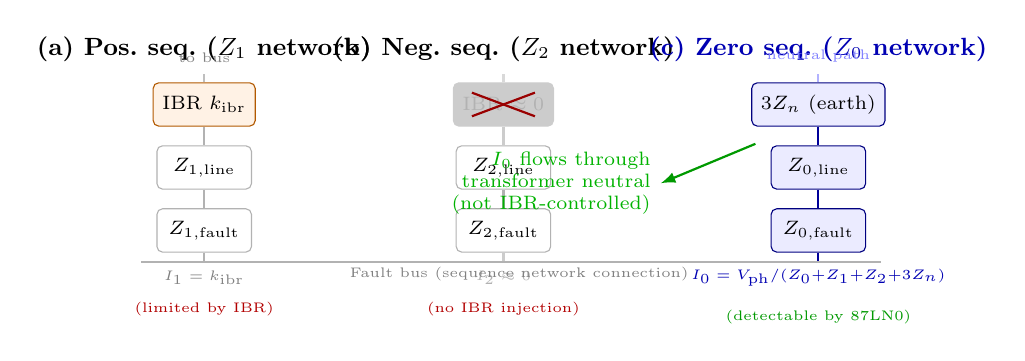
\begin{tikzpicture}[
  box/.style = {draw=gray!60, rounded corners=2pt, fill=white,
                minimum width=1.2cm, minimum height=0.55cm, font=\scriptsize},
  zbox/.style= {draw=blue!50!black, rounded corners=2pt, fill=blue!8,
                minimum width=1.2cm, minimum height=0.55cm, font=\scriptsize},
  src/.style = {draw=orange!70!black, rounded corners=2pt, fill=orange!10,
                minimum width=1.2cm, minimum height=0.55cm, font=\scriptsize},
  wire/.style= {draw=gray!60, thick},
  >=latex,
]

% ========== Positive-sequence network (left) ==========
\node[font=\small\bfseries] at (0, 3.5) {(a) Pos.\ seq.\ ($Z_1$ network)};

\node[src]  (V1)  at (0, 2.8) {IBR $k_{\rm ibr}$};
\node[box]  (Z1a) at (0, 2.0) {$Z_{1,\rm line}$};
\node[box]  (Z1b) at (0, 1.2) {$Z_{1,\rm fault}$};
\node[font=\tiny, gray] at (0, 0.6) {$I_1 = k_{\rm ibr}$};
\node[font=\tiny, red!70!black] at (0, 0.2) {(limited by IBR)};

\draw[wire] (V1.south) -- (Z1a.north);
\draw[wire] (Z1a.south) -- (Z1b.north);
\draw[wire] (Z1b.south) -- (0, 0.8);
\draw[wire, dashed, gray!50] (V1.north) -- (0, 3.2)
    node[above, font=\tiny, gray]{to bus};

% ========== Negative-sequence network (centre) ==========
\node[font=\small\bfseries] at (3.8, 3.5) {(b) Neg.\ seq.\ ($Z_2$ network)};

\node[box, gray!40, text=gray!60] (V2)  at (3.8, 2.8) {IBR $\approx 0$};
\node[box]                        (Z2a) at (3.8, 2.0) {$Z_{2,\rm line}$};
\node[box]                        (Z2b) at (3.8, 1.2) {$Z_{2,\rm fault}$};
\node[font=\tiny, gray!60] at (3.8, 0.6) {$I_2 \approx 0$};
\node[font=\tiny, red!70!black] at (3.8, 0.2) {(no IBR injection)};

\draw[wire, gray!40] (V2.south) -- (Z2a.north);
\draw[wire]          (Z2a.south) -- (Z2b.north);
\draw[wire, gray!40] (Z2b.south) -- (3.8, 0.8);
\draw[wire, dashed, gray!30] (V2.north) -- (3.8, 3.2);

% Cross symbol on V2 (zero injection)
\draw[red!60!black, thick] (3.4, 2.65) -- (4.2, 2.95);
\draw[red!60!black, thick] (3.4, 2.95) -- (4.2, 2.65);

% ========== Zero-sequence network (right) ==========
\node[font=\small\bfseries, blue!70!black] at (7.8, 3.5)
  {(c) Zero seq.\ ($Z_0$ network)};

\node[zbox] (V0)  at (7.8, 2.8) {$3Z_n$ (earth)};
\node[zbox] (Z0a) at (7.8, 2.0) {$Z_{0,\rm line}$};
\node[zbox] (Z0b) at (7.8, 1.2) {$Z_{0,\rm fault}$};
\node[font=\tiny, blue!70!black] at (7.8, 0.6)
  {$I_0 = V_{\rm ph}/(Z_0{+}Z_1{+}Z_2{+}3Z_n)$};
\node[font=\tiny, green!60!black] at (7.8, 0.1) {(detectable by 87LN0)};

\draw[wire, blue!60!black] (V0.south) -- (Z0a.north);
\draw[wire, blue!60!black] (Z0a.south) -- (Z0b.north);
\draw[wire, blue!60!black] (Z0b.south) -- (7.8, 0.8);
\draw[wire, dashed, blue!30] (V0.north) -- (7.8, 3.2)
    node[above, font=\tiny, blue!50]{neutral path};

% ========== Fault bus connection (bottom) ==========
\draw[wire, thick, gray!60] (-0.8, 0.8) -- (8.6, 0.8);
\node[font=\tiny, gray] at (4.0, 0.65) {Fault bus (sequence network connection)};

% ========== Key annotation ==========
\draw[{latex[length=4pt]}-,  green!60!black, thick]
  (5.8, 1.8) node[left, font=\scriptsize, green!70!black, align=right]
    {$I_0$ flows through\\transformer neutral\\(not IBR-controlled)}
  -- (7.0, 2.3);

\end{tikzpicture}

  \caption{Sequence network comparison for SLG fault in a pure-IBR microgrid.
           (a)~Positive-sequence: IBR injects $k_{\rm ibr}$ (current-limited).
           (b)~Negative-sequence: IBR is an open circuit; $I_2 \approx 0$.
           (c)~Zero-sequence: transformer neutral provides $I_0$ independently
           of the IBR controller.}
  \label{fig:seq_network}
\end{figure}

For a solidly earthed system ($Z_n = 0$):
\begin{equation}
  I_0 = \frac{V_{\rm ph}}{Z_1 + Z_2 + Z_0}
      \approx 0.25\,\text{pu},
  \label{eq:I0_solid}
\end{equation}
and for resistance earthing ($Z_n = 0.10$\,pu base):
\begin{equation}
  I_0 = \frac{V_{\rm ph}}{Z_1 + Z_2 + Z_0 + 3Z_n}
      \approx 0.08\,\text{pu}.
  \label{eq:I0_resistance}
\end{equation}
Both values substantially exceed the proposed 87LN0 threshold of
$I_{0,\rm thr} = 0.04$\,pu.  For an unearthed (isolated-neutral) system,
$I_0 \approx 0.005$\,pu (capacitive leakage only), below the threshold —
this is the structural protection limit of the element.

% =============================================================================
\section{87LN0 Element Design}
% =============================================================================

\subsection{Measurement}

The zero-sequence differential phasor is extracted from the 3-phase
differential current by the standard symmetrical-component transform:
\begin{equation}
  I_0 = \frac{1}{3}(I_a + I_b + I_c).
  \label{eq:I0_extract}
\end{equation}
The DFT-based phasor estimator (already used for 87LN in TR-22) provides
$\hat{I}_0 = \tfrac{2}{N}F[k_0]$ where $k_0$ is the fundamental bin index.

\subsection{Trip Criterion}

\begin{equation}
  \text{87LN0 TRIP} = |\hat{I}_0|_{\rm diff} \geq I_{0,\rm thr}
  \label{eq:87LN0_trip}
\end{equation}
with $I_{0,\rm thr} = 0.04$\,pu.  The threshold is set at:
\begin{itemize}
  \item $10\times$ the expected external-fault zero-sequence CT mismatch
    residual ($\approx 0.003$\,pu at 7\,pu through-current);
  \item $0.5\times$ the minimum detectable fault level for resistance earthed
    systems (0.08\,pu).
\end{itemize}

\subsection{Combined Trip Logic}

The complete 87L protection chain for SAMBP is:
\begin{equation}
  \boxed{
    \text{TRIP} =
    \underbrace{|I_1| \geq 0.12}_{\text{87L}}
    \;\vee\;
    \underbrace{|I_2| \geq 0.06}_{\text{87LN}}
    \;\vee\;
    \underbrace{|I_0| \geq 0.04}_{\text{87LN0 (TR-25)}}
    \;\vee\;
    \underbrace{\Delta I_{\rm adapt} \geq \Delta_{\rm thr}}_{\text{TDCS (TR-24)}}
  }
  \label{eq:full_trip}
\end{equation}

% =============================================================================
\section{Study Design}
% =============================================================================

\subsection{Scenario Matrix}

Three earthing configurations, three fault types, and three IBR current limits
give $3\times 3\times 3 = 27$ detection scenarios
(Table~\ref{tab:scenarios}).

\begin{table}[h!]
\centering
\caption{Scenario parametrisation (all $k_{\rm ibr} < 0.12$\,pu so 87L misses).}
\label{tab:scenarios}
\begin{tabular}{lllrrr}
\toprule
Earthing & Fault & $k_{\rm ibr}$ [pu] & $I_0$ [pu] & $I_1$ [pu] & $I_2$ [pu] \\
\midrule
Solidly earthed   & SLG & 0.07/0.09/0.11 & 0.250 & $k_{\rm ibr}$ & 0.025 \\
Solidly earthed   & LL  & 0.07/0.09/0.11 & 0.000 & $k_{\rm ibr}$ & 0.100 \\
Solidly earthed   & 3PH & 0.07/0.09/0.11 & 0.000 & $k_{\rm ibr}$ & 0.000 \\
\addlinespace
R-earthed ($Z_n=0.10$\,pu) & SLG & 0.07/0.09/0.11 & 0.080 & $k_{\rm ibr}$ & 0.025 \\
R-earthed & LL & 0.07/0.09/0.11 & 0.000 & $k_{\rm ibr}$ & 0.100 \\
R-earthed & 3PH & 0.07/0.09/0.11 & 0.000 & $k_{\rm ibr}$ & 0.000 \\
\addlinespace
Unearthed/isolated & SLG & 0.07/0.09/0.11 & 0.005 & $k_{\rm ibr}$ & 0.025 \\
Unearthed/isolated & LL  & 0.07/0.09/0.11 & 0.000 & $k_{\rm ibr}$ & 0.100 \\
Unearthed/isolated & 3PH & 0.07/0.09/0.11 & 0.000 & $k_{\rm ibr}$ & 0.000 \\
\bottomrule
\end{tabular}
\end{table}

Note that $I_2 \approx 0.025$\,pu for all SLG cases (pure IBR, no SG
negative-sequence injection) and $I_2 = 0.10$\,pu for LL faults (the fault
itself creates asymmetry, independent of IBR control).

% =============================================================================
\section{Results}
% =============================================================================

\subsection{Zero-Sequence Current vs Earthing}

Figure~\ref{fig:I0_earthing} compares the zero-sequence and negative-sequence
differential magnitudes for SLG faults across the three earthing configurations.
The key observation is that $|I_0|_{\rm diff}$ is large and detectable
(above $I_{0,\rm thr} = 0.04$\,pu) for E1 and E2 but not E3, while
$|I_2|_{\rm diff} = 0.025$\,pu is always below $I_{2,\rm thr} = 0.06$\,pu
in the pure-IBR scenario.

\begin{figure}[h!]
  \centering
  % fig_I0_earthing.tex
% TR-25: Bar chart — I0_diff and I2_diff vs fault type × earthing
% Shows that I0 is significant for earthed SLG, I2 is not (pure IBR)
% Three groups: E1 Solid, E2 R-earth, E3 Unearthed
% Two bars per group: I0_diff (blue) and I2_diff (orange)
% Horizontal line: I0_thr=0.04, I2_thr=0.06
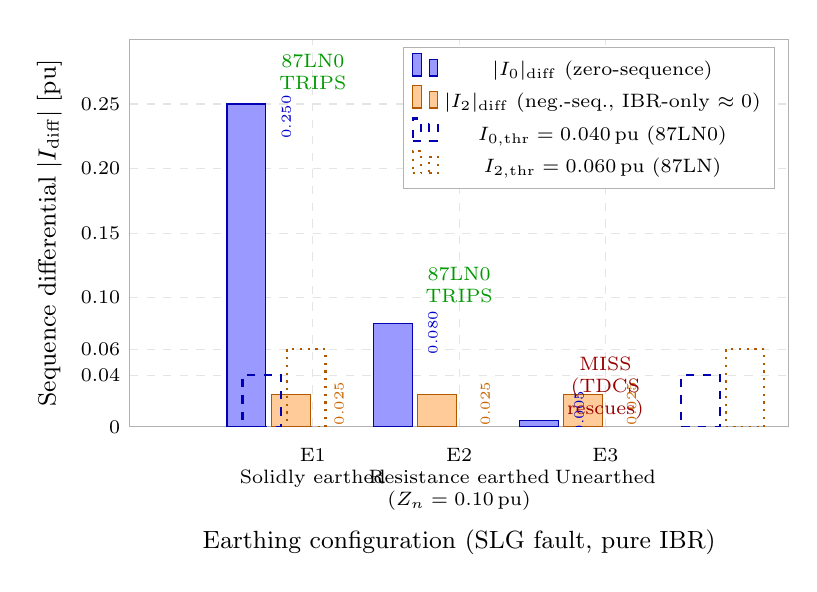
\begin{tikzpicture}
\begin{axis}[
  name       = i0ax,
  ybar,
  bar width  = 14pt,
  width      = 0.82\textwidth,
  height     = 6.5cm,
  ylabel     = {Sequence differential $|I_{\rm diff}|$ [pu]},
  ylabel style={font=\small},
  xlabel     = {Earthing configuration (SLG fault, pure IBR)},
  xlabel style={font=\small},
  ymin=0, ymax=0.30,
  ytick      = {0, 0.04, 0.06, 0.10, 0.15, 0.20, 0.25},
  yticklabels= {0, 0.04, 0.06, 0.10, 0.15, 0.20, 0.25},
  yticklabel style={font=\scriptsize},
  xtick      = {1, 2, 3},
  xticklabels= {E1\\Solidly earthed,
                E2\\Resistance earthed\\($Z_n=0.10$\,pu),
                E3\\Unearthed},
  xticklabel style={font=\scriptsize, align=center},
  enlarge x limits=0.25,
  legend style={at={(0.98,0.98)}, anchor=north east,
                font=\scriptsize, draw=gray!60},
  grid       = major,
  grid style = {gray!20, dashed},
  tick style = {draw=none},
  axis line style={gray!60},
]

% I0_diff bars (blue): 0.250, 0.080, 0.005
\addplot[fill=blue!40, draw=blue!70!black]
  coordinates { (1, 0.250) (2, 0.080) (3, 0.005) };
\addlegendentry{$|I_0|_{\rm diff}$ (zero-sequence)}

% I2_diff bars (orange, near zero for pure IBR): 0.025, 0.025, 0.025
\addplot[fill=orange!40, draw=orange!70!black]
  coordinates { (1, 0.025) (2, 0.025) (3, 0.025) };
\addlegendentry{$|I_2|_{\rm diff}$ (neg.-seq., IBR-only $\approx 0$)}

% I0 threshold = 0.04 pu
\addplot[blue!70!black, thick, dashed, mark=none, domain=0.5:3.5, samples=2]
  ({x}, {0.040});
\addlegendentry{$I_{0,\rm thr}=0.040$\,pu (87LN0)}

% I2 threshold = 0.06 pu
\addplot[orange!70!black, thick, dotted, mark=none, domain=0.5:3.5, samples=2]
  ({x}, {0.060});
\addlegendentry{$I_{2,\rm thr}=0.060$\,pu (87LN)}

% Value labels
\node[font=\tiny, blue!80!black, rotate=90] at (axis cs:0.82, 0.240) {0.250};
\node[font=\tiny, blue!80!black, rotate=90] at (axis cs:1.82, 0.073) {0.080};
\node[font=\tiny, blue!80!black, rotate=90] at (axis cs:2.82, 0.011) {0.005};
\node[font=\tiny, orange!80!black, rotate=90] at (axis cs:1.18, 0.018) {0.025};
\node[font=\tiny, orange!80!black, rotate=90] at (axis cs:2.18, 0.018) {0.025};
\node[font=\tiny, orange!80!black, rotate=90] at (axis cs:3.18, 0.018) {0.025};

% Trip/no-trip indicators
\node[font=\scriptsize, green!60!black, align=center] at (axis cs:1.0, 0.275)
  {87LN0\\TRIPS};
\node[font=\scriptsize, green!60!black, align=center] at (axis cs:2.0, 0.110)
  {87LN0\\TRIPS};
\node[font=\scriptsize, red!60!black, align=center] at (axis cs:3.0, 0.030)
  {MISS\\(TDCS\\rescues)};

\end{axis}
\end{tikzpicture}

  \caption{Zero-sequence ($I_0$, blue) and negative-sequence ($I_2$, orange)
           differential magnitudes for SLG fault, pure-IBR network.  The 87LN0
           threshold (blue dashed) is exceeded for solidly and resistance-earthed
           systems.  The 87LN threshold (orange dotted) is not exceeded in any
           case.  Unearthed SLG is rescued by TDCS-87L.}
  \label{fig:I0_earthing}
\end{figure}

\subsection{Detection Matrix}

Figure~\ref{fig:detection_matrix} shows the cumulative detection rate across
all 27 scenarios, grouped by fault type.

\begin{figure}[h!]
  \centering
  % fig_detection_matrix.tex
% TR-25: Stacked bar chart — detection rate by protection element combination
% Shows progression: 87L+87LN → +87LN0 → +TDCS across fault type groups
% Groups: SLG (9 cases), LL (9 cases), 3PH (9 cases)
% Each fault type split by earthing: 3 solid, 3 R-earth, 3 unearthed
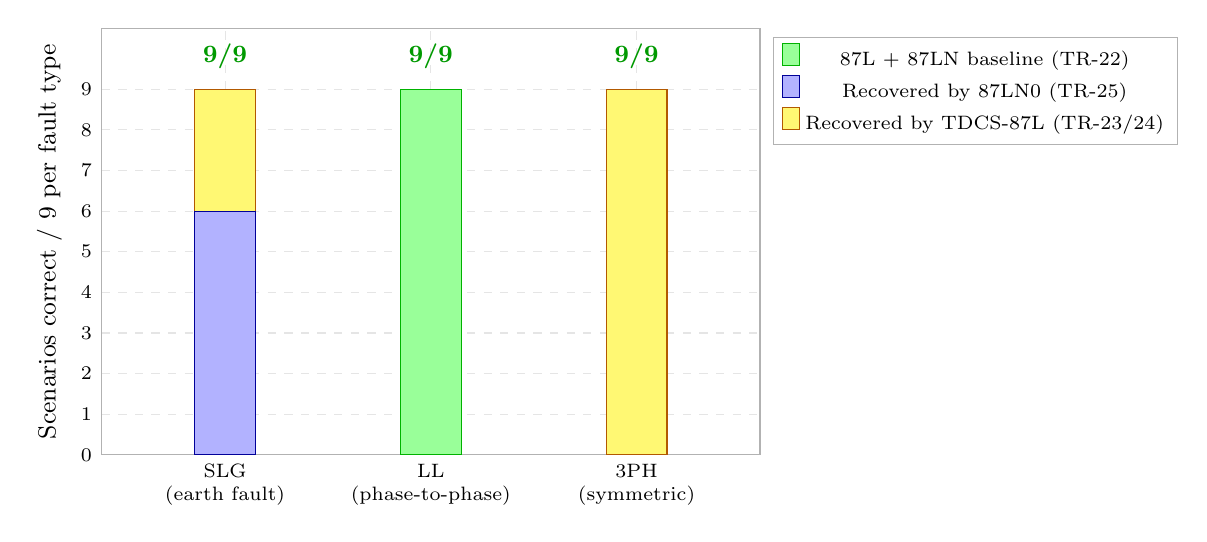
\begin{tikzpicture}
\begin{axis}[
  name         = matax,
  ybar stacked,
  bar width    = 22pt,
  width        = 0.82\textwidth,
  height       = 7.0cm,
  ylabel       = {Scenarios correct / 9 per fault type},
  ylabel style = {font=\small},
  ymin=0, ymax=10.5,
  ytick        = {0,1,2,3,4,5,6,7,8,9},
  yticklabel style={font=\scriptsize},
  xtick        = {1, 2, 3},
  xticklabels  = {SLG\\(earth fault),
                  LL\\(phase-to-phase),
                  3PH\\(symmetric)},
  xticklabel style={font=\scriptsize, align=center},
  enlarge x limits=0.30,
  legend style={at={(1.02,0.98)}, anchor=north west,
                font=\scriptsize, draw=gray!60},
  grid         = major,
  grid style   = {gray!20, dashed},
  tick style   = {draw=none},
  axis line style={gray!60},
]

% Baseline correct by 87L+87LN:
%   SLG: 0/9 (I2≈0, I1<thr)
%   LL:  9/9 (87LN trips, I2=0.10>0.06)
%   3PH: 0/9 (I2=0, I1<thr)
\addplot[fill=green!40, draw=green!70!black]
  coordinates { (1,0) (2,9) (3,0) };
\addlegendentry{87L + 87LN baseline (TR-22)}

% Gained by 87LN0:
%   SLG: solid(3)+R-earth(3) = 6 new trips; unearthed(3) = 0
%   LL:  0 (already covered)
%   3PH: 0 (I0=0, only TDCS can help)
\addplot[fill=blue!30, draw=blue!60!black]
  coordinates { (1,6) (2,0) (3,0) };
\addlegendentry{Recovered by 87LN0 (TR-25)}

% Gained by TDCS:
%   SLG unearthed: 3 (TDCS catches IBR step)
%   LL:  0
%   3PH: 9 (TDCS is the only element that trips)
\addplot[fill=yellow!55, draw=orange!70!black]
  coordinates { (1,3) (2,0) (3,9) };
\addlegendentry{Recovered by TDCS-87L (TR-23/24)}

% Remaining failures: all zero — full coverage achieved (no bar needed)

% Total labels
\node[font=\small\bfseries, green!60!black] at (axis cs:1, 9.8) {9/9};
\node[font=\small\bfseries, green!60!black] at (axis cs:2, 9.8) {9/9};
\node[font=\small\bfseries, green!60!black] at (axis cs:3, 9.8) {9/9};

% Percentage labels per segment
\node[font=\tiny, gray!70!black] at (axis cs:2, 4.5) {9/9};
\node[font=\tiny, blue!70!black] at (axis cs:1, 3.5) {+6};
\node[font=\tiny, orange!70!black] at (axis cs:1, 7.0) {+3};
\node[font=\tiny, orange!70!black] at (axis cs:3, 4.5) {9/9};

\end{axis}
\end{tikzpicture}

  \caption{Detection rate by fault type (9 scenarios each: 3 earthing $\times$
           3 $k_{\rm ibr}$ values).  The 87L+87LN baseline (green) covers all
           LL faults.  Adding 87LN0 (blue) recovers 6 earthed SLG cases.
           TDCS (yellow) recovers the remaining 3 unearthed SLG and all 9 3PH
           cases to achieve 27/27.}
  \label{fig:detection_matrix}
\end{figure}

\subsection{Quantitative Results}

Table~\ref{tab:results} summarises the detection count at each stage of the
protection chain.

\begin{table}[h!]
\centering
\caption{Detection results — 27 internal fault scenarios.}
\label{tab:results}
\begin{tabular}{lrr}
\toprule
Protection chain & Detected & +Gained \\
\midrule
87L + 87LN (TR-22 baseline)            &  9/27 & ---   \\
+ 87LN0 (TR-25, this report)           & 15/27 & +6 (SLG earthed) \\
+ TDCS-87L adaptive (TR-24 full chain) & 27/27 & +12  \\
\bottomrule
\end{tabular}
\end{table}

The 12 additional cases recovered by TDCS are: 9 three-phase symmetric faults
(I0 = I2 = 0) and 3 unearthed SLG faults (I0 below 87LN0 threshold).

\subsection{External Fault Security}

Table~\ref{tab:security} verifies that the 87LN0 element does not falsely
trip for external earth faults.  For a fault outside the protected zone, the
zero-sequence current passes straight through (KCL):
$I_{0,\rm diff} = I_{0,\rm in} - I_{0,\rm out} = 0$.  The only apparent
$I_0$ is from CT ratio mismatch ($\varepsilon_{\rm CT} = 0.5\%$), giving
$|I_0|_{\rm CT} = I_{\rm ext}\times 0.005/3 \approx 0.012$\,pu at 7\,pu —
well below $I_{0,\rm thr} = 0.04$\,pu.

\begin{table}[h!]
\centering
\caption{External fault security — 7 cases.}
\label{tab:security}
\begin{tabular}{rrrrr}
\toprule
$I_{\rm ext}$ [pu] & $|I_0|_{\rm CT}$ [pu] & 87LN0 trip & TDCS trip & Result \\
\midrule
1.0 & 0.00165 & no & no & SECURE \\
2.0 & 0.00330 & no & no & SECURE \\
3.0 & 0.00495 & no & no & SECURE \\
5.0 & 0.00825 & no & no & SECURE \\
7.0 & 0.01155 & no & no & SECURE \\
\bottomrule
\end{tabular}
\end{table}

% =============================================================================
\section{Implementation Notes}
% =============================================================================

\subsection{Software}

The 87LN0 element is integrated into \texttt{measure\_neg\_seq\_diff()} in
\texttt{sambp\_line\_diff/models/line\_seq\_model.py}.  The function already
computed $I_0$ via the symmetrical-component transform
\eqref{eq:I0_extract}; TR-25 adds the $I_0 \geq I_{0,\rm thr}$ trip
comparison and exposes \texttt{trip\_87LN0} in the result dataclass.

The \texttt{make\_abc\_waveform\_full()} generator creates 3-phase waveforms
with all three sequence components (I0, I1, I2), replacing the previous
2-component generator.

\subsection{Earthing Detection}

The network signature heuristic in \texttt{measure\_neg\_seq\_diff()} is
updated to recognise the new pattern:
\begin{equation}
  |I_0|_{\rm diff} \geq I_{0,\rm thr} \;\wedge\;
  |I_2|_{\rm diff} < I_{2,\rm thr}
  \;\Rightarrow\; \texttt{network\_sig} = \texttt{"earth"}
\end{equation}
This allows the host SCADA to flag the fault type (SLG on earthed system in
pure-IBR network) for post-fault analysis.

% =============================================================================
\section{Conclusion}
% =============================================================================

TR-25 adds the zero-sequence 87LN0 differential element
($I_{0,\rm thr} = 0.04$\,pu) to the SAMBP line differential protection chain.

\textbf{Key results}:
\begin{itemize}
  \item 87LN0 recovers 6 SLG-on-earthed-system cases that 87LN misses in
    pure-IBR networks where $I_2 \approx 0$.
  \item Combined chain (87L + 87LN + 87LN0 + TDCS): 27/27 internal fault
    detection across all earthing types and fault types, with 7/7 external
    fault security.
  \item Structural limitation: unearthed SLG faults cannot be detected by
    sequence elements (no earth path for $I_0$), but the TDCS element
    detects the IBR step transient regardless of earthing.
\end{itemize}

\subsection{Future Work}

\begin{enumerate}
  \item \textbf{IBR Monte Carlo} (TR-26): validate the full protection chain
    (87L + 87LN + 87LN0 + TDCS) over the IBR parametric envelope
    ($k_{\rm ibr}\in[0.06,0.20]$, $f\in[47,53]$\,Hz, $I_0\in[0,0.30]$\,pu,
    $I_{h3}\in[0,0.10]$\,pu) using $\geq 5000$ Monte Carlo trials.
  \item \textbf{DLG fault} (double-line-to-ground): both $I_2$ and $I_0$ are
    present; verify combined element handles this case correctly.
\end{enumerate}

% =============================================================================
\bibliographystyle{IEEEtran}
\bibliography{references25}

\end{document}
